\documentclass[a4j, dvipdfmx]{jsarticle}

\usepackage[a4paper, left=2.0cm, right=2.0cm, top=2.0cm, bottom=2.0cm]{geometry}
\usepackage{amsmath}
\usepackage[dvipdfmx]{graphicx}
\usepackage{amssymb}
\usepackage{booktabs}
\usepackage{array}

\newcolumntype{P}[1]{>{\raggedright\arraybackslash}p{#1}}

% 小見出し（\paragraph）の先頭に付く■を消す
\renewcommand{\jsParagraphMark}{}

% 指標名（周りの文章と同じ字体・太さで出すため，数式ではなく文章の書体で組む）
\newcommand{\PushRatio}{\textrm{push\_ratio}}
\newcommand{\Spread}{\textrm{spread}}
\newcommand{\Push}{\textrm{push}}

\title{
Federated Learningにおける
悪性更新の検知可能性の評価\\[0.8em]
\large
― データ分布の不均一性と攻撃のステルス性を軸として ―
}
\author{3CDA2216 笠原秀星}
\date{\today}

% 概要（タイトルの下に段組をまたいで置く）
\makeatletter
\g@addto@macro\@maketitle{%
  \begin{center}
  \begin{minipage}{0.9\textwidth}
  \small
  \textbf{概要}\quad
  Federated Learning（FL）では, 悪性クライアントが送る更新によってグローバルモデルが汚染されうる. 本研究では, 悪性更新の検知を, 集約の直前の更新ベクトルに対する二値分類として捉え, データ分布の不均一性（Non-IID度）と攻撃のステルス性を変えながら, 4種類の検知器の検知性能をROC-AUCにより評価した. その結果, 検知器の優劣は攻撃によって入れ替わり, Non-IIDによる検知性能の低下は, 正常更新のばらつきの大きさではなく, その配分と対応していた. また, 高次元の正常更新は平均からほぼ一定の距離に並ぶため, 平均に近い悪性更新はむしろ目立った. これらの結果から, 悪性更新の押し出し量と正常更新のばらつきの比で検知可能性がほぼ決まるという中心仮説は支持されず, 検知可能性は, 検知器が見る量の上での悪性更新の位置と, 正常更新の分布の形に依存することが示唆された.
  \par\vspace{0.5em}
  \textbf{キーワード}\quad Federated Learning, モデルポイズニング攻撃, 悪性更新検知, Non-IID
  \end{minipage}
  \end{center}
  \vspace{0.5em}%
}
\makeatother

\begin{document}

\maketitle

\section{はじめに}

Federated Learning（以下, FL）は, 生データを共有することなく複数のクライアントが協調してモデルを学習する分散学習の枠組みである\cite{mammen2021fl}. 一方で, FLには悪意のあるクライアントがモデル更新を改ざんするModel Poisoning Attackの脅威がある\cite{sagar2023survey}. 特にALIE\cite{baruch2019little}のように, 悪性更新を正常更新のばらつきの範囲内に収めるステルス攻撃は, Robust Aggregationをもすり抜ける.

攻撃と防御の攻防は, 各ラウンドでサーバが集約を行う直前の更新ベクトル空間で生じている. そこで本研究では, 防御を悪性更新と正常更新を識別する二値分類問題として捉え, 4種類の検知器の検知性能を, 最終精度とは切り離して更新ベクトルに対するROC-AUCで評価する.

先行研究の多くは, 防御の効果を最終精度や攻撃成功率で評価している. Liら（2023）\cite{li2023experimental}はALIEを含む攻撃をIIDとNon-IIDの双方で比較し, Non-IIDでは頑健性が大きく低下することを示したが, その評価は最終精度によるものであった. これに対し, 本研究の新規性は次の3点にある.
\begin{itemize}
  \item 悪性更新の見分けやすさを, 集約の直前の更新ベクトルに対するROC-AUCで, 学習のラウンドごとに評価する.
  \item データ分布の不均一性（Non-IID度）と攻撃のステルス性の2つを同時に変え, 検知が破綻する条件を調べる.
  \item Non-IIDによる検知性能の低下を, 悪性更新の押し出し量と正常更新のばらつきの比（push\_ratio）, および正常更新の分布の形の観点から説明することを試みる.
\end{itemize}

本研究の結果, 検知可能性は \PushRatio{} ではほぼ決まらず, 検知器が見る量の上での悪性更新の位置と, 正常更新の分布の形に依存することが示唆された.

\section{関連研究}

Sagarらは, FLにおけるPoisoning Attackおよび防御手法に関する包括的なサーベイを行っている. 彼らは攻撃をData Poisoning AttackとModel Poisoning Attackに分類し, 防御手法についてもRobust Aggregationや異常検知手法などの観点から体系的に整理している\cite{sagar2023survey}.

Fangらは, Byzantine-robustなFLに対するLocal Model Poisoning Attackを提案した. 攻撃を最適化問題として定式化することで, Krum, Bulyan, Median, Trimmed MeanといったByzantine-robust Aggregation手法に対しても有効な攻撃を実現し, 既存の防御手法が十分ではないことを示した\cite{fang2020local}.

Robust Aggregationの基礎としては, BlanchardらのKrum\cite{blanchard2017krum}, Yinらの座標ごとMedian/Trimmed Mean\cite{yin2018byzantine}, El MhamdiらのBulyan\cite{elmhamdi2018hidden} がある. これらは一定割合以下のByzantineクライアントに対する理論的保証を与えるが, いずれも「正常更新が互いに近い」ことを暗に仮定しており, Non-IID環境では保証が弱まる.

Baruchらは, 正常更新の座標ごとの標準偏差の範囲内に収まる小さな摂動を悪性クライアント全員が協調して送る``A Little Is Enough''（ALIE）攻撃を提案し, Trimmed Mean, Krum, Bulyanを回避できることを示した\cite{baruch2019little}. Shejwalkarらは, 集約手法非依存のmin-max/min-sum攻撃と, 特異値分解に基づく検知（Divide-and-Conquer）を提案した\cite{shejwalkar2021manipulating}.

検知型防御としては, コサイン距離のクラスタリングと重みクリッピングを組み合わせるFLAME\cite{nguyen2022flame}がある.

データ分布の不均一性の扱いとしては, Hsuらのディリクレ分布によるラベル分割\cite{hsu2019measuring} が標準的であり, NIID-Bench\cite{li2022federated} が各種分割方式を体系的に比較している.

本研究に特に近い2つの先行研究がある. Liら（2023）は, FedSGD/FedAvg上で8種のRobust Aggregation手法と5種のByzantine攻撃（ALIE等を含む）をIID/Non-IID双方で比較する実験的研究を行い, Non-IIDデータでは全手法の頑健性が大きく低下し, 一部は悪性クライアントが皆無でも性能が悪化することを示した\cite{li2023experimental}. ただし彼らの評価指標は最終精度であり, 学習の過程で頑健性がどう変化するかは扱っていない. また, Wangらは, コサイン類似度・$L_2$ノルム・ユークリッド距離といった類似度指標が高次元パラメータ空間では, パラメータの値が大きく異なっていても類似と評価されうるという欠点を持つことを示し, この欠点を突く攻撃Fakerを提案した\cite{wang2023trust}. この結果は, コサイン距離に基づく検知器（本研究のD2に相当）が攻撃によって欺かれうることを示している.

これらの研究の多くは, 最終精度や攻撃成功率によって評価するか, 検知性能を単一のNon-IID水準でのみ報告している. なお, 本研究はNon-IID環境に最適化された新しい攻撃を提案するものではなく, 検知性能と正常更新のばらつきの関係を分析するものである.

\section{研究の問いと仮説}
\label{sec:rq}

\subsection{研究の問い}

本研究では, 次の3つの問いを明らかにする. 第一に, FLにおける悪性更新は更新ベクトルレベルの異常検知でどの程度見分けられるか, また検知性能は集約手法に依存しない代表的な検知器の間でどう異なるか. 第二に, データ分布の不均一性（Non-IID度）は検知性能をどう低下させるか, またその低下は正常更新のばらつきの増大によって説明できるか. 第三に, 攻撃のステルス性, すなわち悪性更新を正常クラスタ内に収める度合いは検知性能をどう左右するか, また検知が破綻する境界はどこにあるか.

\subsection{中心仮説}

\begin{quote}
悪性更新が検知可能かどうかは, 悪性更新の押し出し量が正常クライアント間のばらつきを超えているかでほぼ決まる. Non-IIDは正常更新のばらつきを増大させるため, 攻撃を正常な多様性の中へ紛れ込ませ, 検知性能を低下させる.
\end{quote}

この仮説を検証するための説明変数として, 正常クラスタの広がり \Spread{}, 悪性更新の押し出し距離 \Push{}, およびその比 \PushRatio{}（\ref{sec:metrics}節で定義）を導入する. 仮説が正しければ, 検知性能（ROC-AUC）は \PushRatio{} が $1$ を下回る領域で急落し, Non-IID度が強いほど同じ攻撃強度でも \PushRatio{} が小さくなる, という関係が観測されるはずである. ただし, ALIE（A2）では \PushRatio{} が構成上ほぼ $z$ に等しく, Non-IID度によって変化しない（\ref{sec:attacks}節）. このため, \PushRatio{} とAUCの観測上の関係は符号反転攻撃（A1）で調べ, A2は $z$ によって \PushRatio{} を $1$ の上下に動かす条件, および \PushRatio{} を一定に保ったままNon-IID度だけを変える条件として用いる.

\section{脅威モデル}
\label{sec:threat}

本研究では, 攻撃者と防御者について次の脅威モデルを仮定する. 攻撃者はfull knowledgeを持つものとする. すなわち, 悪性クライアントは各ラウンドで正常クライアントの更新を参照でき, 互いに結託できる. 本実験では, この攻撃者をサーバ側で模擬する. 悪性クライアントの集合は全ラウンドを通じて固定し, その割合は $f/n \le 0.3$ を想定し, 本実験では $f/n = 0.2$ とする.

防御者はサーバ側に位置し, 全クライアントの更新ベクトルを観測できるが, クリーンなデータは持たない. したがって, FLTrust\cite{cao2021fltrust}のように, サーバが少量のクリーンなデータを持ち, それを信頼の基準とする防御は対象外とする. また, どのクライアントが悪性かという正解ラベルは評価にのみ用い, 検知器には一切与えない.

この脅威モデルは攻撃者に有利な楽観的設定である. Shejwalkarら\cite{shejwalkar2022back}は現実的な制約下ではpoisoningの脅威が限定的であると論じているが, 本研究は「検知性能の上限」を評価するものとして位置づける.

\section{評価枠組み}
\label{sec:framework}

\subsection{記法}

通信ラウンド $t$ において, 参加クライアント $i \in \{1,\dots,n\}$ のモデル更新ベクトルを $g_i = w_i - w_{\text{global}}$ とする. 正常クライアントの添字集合を $B$, 悪性クライアントの添字集合を $M$（$|M| = f$）とし, $\bar{g}_B = \frac{1}{|B|}\sum_{i \in B} g_i$ を正常更新の平均とする. 集約にはFedAvg\cite{mcmahan2017fedavg}を用い, 毎ラウンド全クライアントの更新を各クライアントのデータ数で重み付けして平均する.

\subsection{検知器}
\label{sec:detectors}

本研究では, 集約手法に依存しない汎用的な4種の検知器D1--D4を用いる. いずれの検知器も, 各クライアント $i$ に異常スコア $s_i$（大きいほど悪性らしい）を与える.

\paragraph{D1: ノルム偏差}
\begin{equation}
s_i = \left|\; \|g_i\|_2 - \operatorname*{median}_{j}\|g_j\|_2 \;\right|
\end{equation}
偶数台のクライアントでは, 中央値を挟む2台のスコアは定義上等しくなるため, 数値誤差によらず同値として扱う. D1は最も単純な検知器であり, ノルムを大きく変える攻撃（スケーリングやランダムノイズ）の検知には有効だが, ステルス攻撃には弱いと予想される. FLAME\cite{nguyen2022flame}などの重みクリッピング系の防御に対応する.

\paragraph{D2: 参照方向へのコサイン距離}
座標ごとの中央値 $r = \operatorname{median}(g_1,\dots,g_n)$ を参照方向とし,
\begin{equation}
s_i = 1 - \frac{g_i \cdot r}{\|g_i\|_2\,\|r\|_2}.
\end{equation}
D2は更新の向きの異常を捉える検知器であり, FLAME\cite{nguyen2022flame}の考え方に対応する.

\paragraph{D3: 2クラスタリング}
各更新のノルム $\|g_i\|_2$, D2スコア, および第1・第2主成分への射影の4つを特徴量 $\phi_i$ とし, 特徴量ごとに標準化したうえで $k$-means（$k=2$）を適用し, 大きい方のクラスタを正常とみなして, その重心までの距離をスコアとする. 初期中心は全ての2点の組を試し, クラスタ内平方和が最小となる分割を採用する. Auror\cite{shen2016auror}の考え方に対応する.

\paragraph{D4: スペクトル残差}
各更新を中心化した $\tilde{g}_i = g_i - \frac{1}{n}\sum_{k=1}^{n} g_k$ を並べた行列 $\tilde{G} = [\tilde{g}_1;\dots;\tilde{g}_n]$ の第1右特異ベクトル $v$ を求め,
\begin{equation}
s_i = (\tilde{g}_i \cdot v)^2
\end{equation}
とする. D4はSpectral Signatures\cite{tran2018spectral}やDivide-and-Conquer\cite{shejwalkar2021manipulating}の考え方に対応する.

\subsection{攻撃}
\label{sec:attacks}

\paragraph{A1: 符号反転攻撃}
\begin{equation}
g_i^{\text{mal}} = -\,g_i \qquad (i \in M)
\end{equation}
各悪性クライアントは自身のローカルデータで正常に学習した更新 $g_i$ の符号を反転して送る. 向きは自身の正常更新と正反対になる一方, ノルムは変わらない. A1は, 向きに基づく検知器であれば容易に検知できるはずの粗い攻撃であり, ベースラインとして用いる.

\paragraph{A2: ALIE}
本研究では, Baruchら\cite{baruch2019little}が提案したALIE（A Little Is Enough）の更新生成則を用いる. 攻撃者は当該ラウンドの正常クライアントの更新から座標ごとの平均 $\mu$ と標準偏差 $\sigma$ を求め,
\begin{equation}
g_i^{\text{mal}} = \mu - z\,\sigma \qquad (i \in M)
\label{eq:alie}
\end{equation}
とし, 悪性クライアントは全員この同一のベクトルを送る. 原論文は $\mu$ と $\sigma$ を悪性ワーカー自身のデータから推定するが, 本研究では正常クライアントの更新そのものから求めており, 原論文より強い攻撃者を想定している.

$z$ は $0.385$, $0.5$, $0.75$, $1$, $1.25$, $1.5$, $2$, $3$ の8水準とする. 最小の $0.385$ は, 原論文が正規分布の仮定の下で定めた摂動の上限 $z_{\max}$ を本研究の $n=20,\ f=4$ に当てはめた値であり, Non-IID環境での理論的な上限ではなく参照値として用いる. 原論文もMNISTで $z=1.5$ を用いるなど, $z_{\max}$ より大きい $z$ を用いている. なお, 原論文における「検知されない」とは, Trimmed Meanで除外されないこと, およびKrumで選択されることを指し, 更新ベクトル全体として正常更新と区別できないことを意味するものではない. また, Non-IID環境では正常更新が原論文の分布の仮定を満たすとは限らないため, 本研究はALIEの理論的保証を仮定せず, 同一の生成則を異なるNon-IID条件へ適用して検知性能を比較する.

ALIEでは, \PushRatio{}（\ref{sec:metrics}節）が構成上ほぼ定まる. $\mu$ は正常更新の平均 $\bar{g}_B$ に等しく, $\sigma$ を母標準偏差とし, $d_i = \|g_i - \bar{g}_B\|_2$ とおくと,
\begin{equation}
\PushRatio
= z \cdot \frac{\sqrt{\frac{1}{|B|}\sum_{i \in B} d_i^2}}{\frac{1}{|B|}\sum_{i \in B} d_i}
\;\ge\; z
\label{eq:alie-pushratio}
\end{equation}
となる. すなわち, $z$ を固定したA2では, Non-IID度が異なる条件の間でも \PushRatio{} がほぼ一定に保たれる.

\subsection{データ分布（Non-IID）}
\label{sec:data-noniid}

ディリクレ分布によるラベル分割\cite{hsu2019measuring}を用いる. クライアント $k$ ごとにクラスの比率 $q_k \sim \mathrm{Dir}(\alpha \pi)$ を引き, その比率に従って全クライアントに同数（$1{,}500$ 件）のデータを配る. ここで $\pi$ は学習データ全体におけるクラスの比率である. $\alpha$ を大きくするとどのクライアントの比率も $\pi$ に近づき（IID）, 小さくすると各クライアントの保有クラスが偏る. 本研究では $\alpha \in \{1000\;(\approx\text{IID}),\; 5,\; 1\}$ の3水準を用いる. クライアントが最も多く保有するクラスの割合は, 10試行の平均で $\alpha=1000,\ 5,\ 1$ の順に $12\%,\ 38\%,\ 65\%$ である. 配るデータの合計は学習データ $60{,}000$ 件の半分の $30{,}000$ 件とし, 各クライアントは配られたデータの8割（$1{,}200$ 件）をローカル学習に用いる.

Non-IIDには, ラベル分布の偏り, 特徴分布の偏り, データ数の偏りなどの種類がある\cite{li2022federated}. このうち本研究の「Non-IID度」はラベル分布の偏りのみを指す. データ数を全クライアントで等しくしたのは, データ数が不均一だと更新のノルムやFedAvgの重みが変わり, 検知性能の変化がラベル分布の偏りによるものかを切り分けられないためである.

\subsection{検知性能の評価指標}
\label{sec:roc-auc}

異常検知器は各サンプルに異常スコア $s$（大きいほど異常らしい）を与える. 閾値を $+\infty$ から $-\infty$ まで動かしたときの偽陽性率と真陽性率の組 $(\mathrm{FPR}, \mathrm{TPR})$ の軌跡をROC曲線と呼び, その下側の面積をROC-AUC（以下AUC）と呼ぶ\cite{fawcett2006roc}. AUCは次の確率的な解釈を持つ\cite{hanley1982meaning}. 悪性（陽性）の集合を $M$, 正常（陰性）の集合を $B$ とすると,
\begin{equation}
\mathrm{AUC}
= \frac{1}{|M|\,|B|}\sum_{i \in M}\sum_{j \in B}
\Bigl( \mathbf{1}[s_i > s_j] + \tfrac{1}{2}\,\mathbf{1}[s_i = s_j] \Bigr)
\label{eq:auc}
\end{equation}
であり, これは「ランダムに選んだ悪性サンプルのスコアが, ランダムに選んだ正常サンプルのスコアを上回る確率」に等しい. $\mathrm{AUC}=1$ は完全な分離, $\mathrm{AUC}=0.5$ はランダムな順位付けと同等であり, $\mathrm{AUC}<0.5$ は検知器が悪性を正常より「正常らしい」と評価していることを意味する. AUCは閾値の選び方に左右されず, 悪性が少数派の不均衡な設定でもクラス比の影響を受けにくいため, 検知器が悪性と正常を分離できているかの評価に適している.

\subsection{評価指標}
\label{sec:metrics}

各ラウンド $t$ では, 全クライアントについて異常スコアと悪性ラベルの組 $(s_i, y_i)$ が得られる（$y_i = 1$ なら悪性）. 検知性能の指標には閾値に依存しないROC-AUC（定義は\ref{sec:roc-auc}節）を用いる. AUCはラウンドごとに算出し, AUCのラウンド推移を示すとともに, 条件ごとに要約する. 要約では, 同じ実行の中のラウンドどうしは独立でないため, 試行ごとに第46--50ラウンドのAUCを平均してから, 試行間の平均と標準偏差を求める.

中心仮説を検証するための説明変数として, 正常更新の平均からの距離の平均 \Spread{}, 悪性更新の正常更新の平均からの距離の平均 \Push{}, およびその比 \PushRatio{} を次のように定義する.
\begin{align*}
  \Spread &= \tfrac{1}{|B|}\textstyle\sum_{i \in B}\|g_i - \bar{g}_B\|_2, \\
  \Push   &= \tfrac{1}{|M|}\textstyle\sum_{i \in M}\|g_i - \bar{g}_B\|_2, \\
  \PushRatio &= \Push\,/\,\Spread.
\end{align*}

\PushRatio{} とAUCの関係は, 符号反転攻撃について, 検知器ごとにSpearman順位相関係数 $\rho$ で評価する. 符号反転の \PushRatio{} は主に $\alpha$ によって変わるため, 全体の相関に加えて $\alpha$ ごとの相関も求める. $\rho$ は直線関係を仮定せず外れ値の影響も受けにくいため, 値が桁単位で変化する \PushRatio{} と, 上限1で頭打ちになるAUCとの関係の評価に適している. 同順位は平均順位で処理する. ALIEについては, 横軸を $z$ としたAUCの図を $\alpha$ ごとに示す.

さらに, 同じ \Spread{} でも正常更新の広がり方によって検知の難しさが異なりうるため, 正常更新の分布構造を表す次の2つの指標を各ラウンドで記録する. これらは正解ラベルを用いる考察用の説明変数であり, 検知器には与えない. 第一に, 中心化した正常更新の行列の特異値 $\{\sqrt{\lambda_k}\}$ から第1主成分の寄与率 $\lambda_1 / \sum_k \lambda_k$ を求める. これは正常更新が特定の方向へ集中している度合いを表し, D4が実際に用いる, 悪性を含む全更新についても同じ量を求める. 第二に, 悪性方向 $a = \bar{g}_M - \bar{g}_B$（$\bar{g}_M$ は悪性更新の平均）と第1主成分 $v_1$ のなす角について $|\cos\theta| = |a \cdot v_1| / (\|a\|_2\,\|v_1\|_2)$ を, 正常更新のみの第1主成分と全更新の第1主成分（D4の射影方向）の両方に対して求める.

\section{実験}
\label{sec:experiment}

\subsection{実験環境と学習設定}
\label{sec:exp-setting}

学習・環境設定を表\ref{tab:exp-setting}に, 実験条件を表\ref{tab:exp-conditions}に示す. モデルにはFangら\cite{fang2020local}に準拠した小型CNNを用いる. ローカルエポック数を2としたのは, 1台あたりの学習データが $1{,}200$ 件と少なく, 1エポックでは50ラウンドで学習が十分に進まなかったためである. ただし, この設定でも $\alpha=1$ の学習は50ラウンドの時点で収束していない（\ref{sec:res-acc}節）. 検知性能はラウンドによって変化しうるため（\ref{sec:res-rounds}節）, 条件の代表値には第46--50ラウンドの値を用い, ラウンド推移を併せて示す.

\begin{table}[t]
\centering
\begin{minipage}[t]{0.51\textwidth}
\centering
\caption{学習・環境設定}
\label{tab:exp-setting}
\small
\begin{tabular}{@{}l@{\hspace{0.8em}}P{5.4cm}@{}}
\toprule
項目 & 値 \\
\midrule
データセット & MNIST（10クラス分類） \\
モデル & 小型CNN（Fang準拠） \\
クライアント数 $n$ & 20（毎ラウンド全参加） \\
1台あたりのデータ & $1{,}500$ 件（学習 $1{,}200$ 件） \\
通信ラウンド数 & 50 \\
ローカルエポック数 & 2 \\
バッチサイズ & 32 \\
学習率 & $0.01$ \\
最適化 & SGD（モーメンタムなし） \\
集約 & FedAvg \\
実装 & PyTorch / Flower（シミュレーション） \\
実行環境 & CPU \\
\bottomrule
\end{tabular}
\end{minipage}\hfill
\begin{minipage}[t]{0.47\textwidth}
\centering
\caption{実験条件}
\label{tab:exp-conditions}
\small
\begin{tabular}{@{}lP{5.6cm}@{}}
\toprule
軸 & 水準 \\
\midrule
Non-IID度 $\alpha$ & $1000,\; 5,\; 1$ \\
攻撃 & 符号反転（A1）, ALIE（A2, $z=0.385,\ 0.5,\ 0.75,\ 1,$ $1.25,\ 1.5,\ 2,\ 3$） \\
悪性割合 $f/n$ & $0.2$（固定, $f=4$） \\
検知器 & D1--D4 \\
試行数 & $10$ \\
\bottomrule
\end{tabular}
\end{minipage}
\end{table}

\subsection{実験条件}
\label{sec:exp-conditions}

攻撃ありの条件は $3\,(\alpha) \times 9\,(\text{攻撃}) \times 10\,(\text{試行}) = 270$ 回であり, これに加えて, \Spread{} と精度の基準値を得るため, 攻撃なしの条件を $30$ 回実行した（計 $300$ 回）. 悪性クライアントの集合は各試行の中で全ラウンドを通じて固定し, 試行番号をデータ分割, モデルの初期値, ローカル学習時のデータの並べ替え, および悪性クライアントの選出の乱数に対応させた. これにより, 同じ番号の試行では $\alpha$ と攻撃によらず同じ4台が悪性クライアントとなる.

\subsection{実装と計測}
\label{sec:exp-impl}

実験系は, Flower\cite{beutel2020flower}のシミュレーション機能を用い, 1台の計算機の上に20台のクライアントを仮想的に立てて構築した. 符号反転攻撃（A1）は, 悪性クライアントの中で, 学習で得た更新量の符号を反転してから返す形で実装した. サーバ側では, FedAvgの戦略を拡張し, 全クライアントの返信がそろった後, 集約の前に次の処理を挟んだ. まず, ALIE（A2）の場合は, 正常クライアントの更新から座標ごとの平均と標準偏差を求め, 悪性クライアントの更新を式(\ref{eq:alie})のベクトルに差し替える. これは第\ref{sec:threat}章の脅威モデルをサーバ側で模擬するためである. 次に, 攻撃適用後の更新ベクトル集合に4種の検知器を適用し, スコア, ROC-AUC, \Spread{}, \Push{}, \PushRatio{}, および分布構造の指標をラウンドごとに記録する. 悪性ラベルは評価と分布構造の指標の算出にのみ用い, 検知器には与えない. 最後に, 検知結果を用いずにFedAvgで集約する. あわせて, グローバルモデルのテスト精度をラウンドごとに記録した.

\section{実験結果}
\label{sec:results}

300回の実行（攻撃あり270回, 攻撃なし30回）はすべて表\ref{tab:exp-setting}・表\ref{tab:exp-conditions}の設定どおりに50ラウンドを完了した. 以下, 表中の値は特に断らない限り試行間の平均である.

\subsection{学習の収束と攻撃が精度に与える影響}
\label{sec:res-acc}

表\ref{tab:acc}に第50ラウンドにおけるグローバルモデルのテスト精度を, 図\ref{fig:acc-round}に精度のラウンド推移を示す.

\begin{table*}[t]
\centering
\caption{第50ラウンドのテスト精度 [\%]（10試行の平均$\pm$標準偏差）と, 第45ラウンドから第50ラウンドまでの精度の上がり幅 [ポイント]（10試行の平均）}
\label{tab:acc}
\small
\begin{tabular}{@{}lcccccc@{}}
\toprule
 & \multicolumn{3}{c}{第50ラウンドの精度} & \multicolumn{3}{c}{第45--50ラウンドの上がり幅} \\
\cmidrule(lr){2-4}\cmidrule(l){5-7}
攻撃 & $\alpha=1000$ & $\alpha=5$ & $\alpha=1$ & $\alpha=1000$ & $\alpha=5$ & $\alpha=1$ \\
\midrule
攻撃なし & $98.02 \pm 0.11$ & $97.43 \pm 0.24$ & $94.30 \pm 1.25$ & 0.14 & 0.17 & 0.53 \\
A1 符号反転 & $97.09 \pm 0.20$ & $95.03 \pm 1.01$ & $76.25 \pm 7.84$ & 0.16 & 0.26 & 0.05 \\
\midrule
A2 $z{=}0.385$ & $98.00 \pm 0.10$ & $97.29 \pm 0.25$ & $92.94 \pm 2.47$ & 0.13 & 0.16 & 0.63 \\
A2 $z{=}0.5$ & $97.99 \pm 0.08$ & $97.29 \pm 0.25$ & $92.89 \pm 2.50$ & 0.14 & 0.16 & 0.64 \\
A2 $z{=}0.75$ & $98.01 \pm 0.08$ & $97.29 \pm 0.26$ & $92.78 \pm 2.57$ & 0.13 & 0.17 & 0.69 \\
A2 $z{=}1$ & $98.01 \pm 0.10$ & $97.28 \pm 0.25$ & $92.63 \pm 2.69$ & 0.14 & 0.16 & 0.65 \\
A2 $z{=}1.25$ & $98.00 \pm 0.11$ & $97.27 \pm 0.25$ & $92.47 \pm 2.74$ & 0.12 & 0.16 & 0.63 \\
A2 $z{=}1.5$ & $98.00 \pm 0.11$ & $97.24 \pm 0.26$ & $92.35 \pm 2.69$ & 0.13 & 0.12 & 0.67 \\
A2 $z{=}2$ & $97.96 \pm 0.10$ & $97.19 \pm 0.26$ & $91.75 \pm 2.78$ & 0.13 & 0.14 & 0.70 \\
A2 $z{=}3$ & $97.86 \pm 0.11$ & $96.97 \pm 0.31$ & $89.11 \pm 3.28$ & 0.11 & 0.15 & 0.88 \\
\bottomrule
\end{tabular}
\end{table*}

\begin{figure*}[t]
\centering
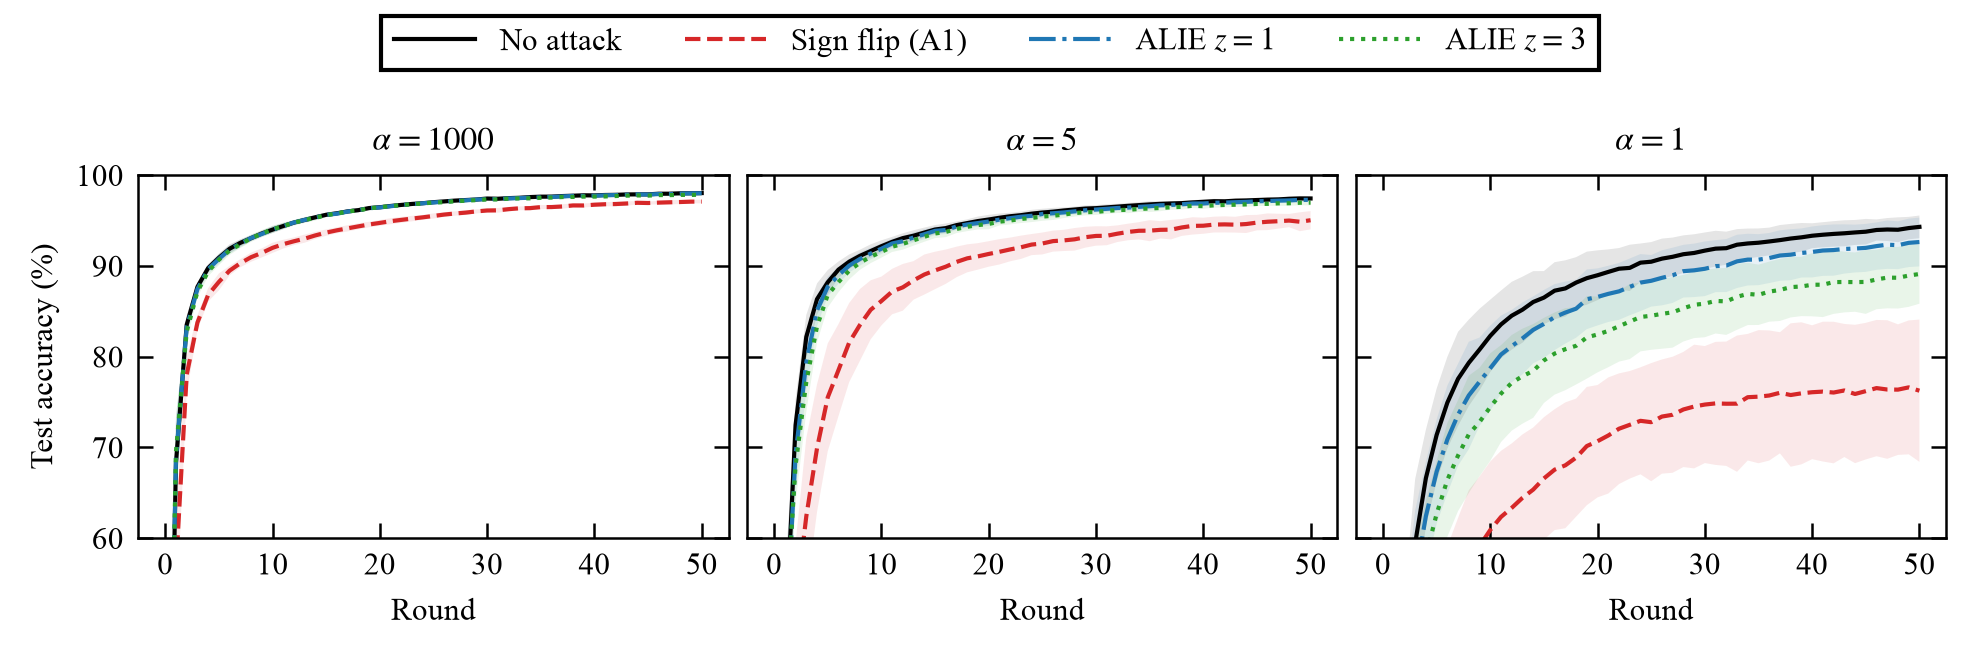
\includegraphics[width=0.75\textwidth]{fig/accuracy_by_round_v3.png}
\caption{テスト精度のラウンド推移（10試行の平均, 帯は$\pm$標準偏差）. ALIEは8水準の $z$ のうち $z=1$ と $z=3$ のみを示す. 縦軸は $60\%$ 以上を表示}
\label{fig:acc-round}
\end{figure*}

攻撃なしの条件の精度は $\alpha=1000,\,5,\,1$ でそれぞれ $98.0\%$, $97.4\%$, $94.3\%$ であった. ただし, $\alpha=1$ では第45--50ラウンドでも精度が $0.5$ ポイント程度上昇しており, $\alpha=1$ の第46--50ラウンドの検知性能は, 学習が進みきる前の段階のものである. 符号反転は精度を $\alpha=1000,\,5$ でそれぞれ約 $0.9$, $2.4$ ポイント, $\alpha=1$ で約 $18$ ポイント低下させた. 一方, ALIEは $\alpha=1000,\,5$ ではどの $z$ でも攻撃なしとの差が最大 $0.5$ ポイントであり, $\alpha=1$ でも $z \le 1.5$ では2ポイント以内であった.

\subsection{検知性能の全体像}
\label{sec:res-final}

表\ref{tab:final-auc}に, 第46--50ラウンドのROC-AUCを, 図\ref{fig:auc-z}にALIEの $z$ とAUCの関係を示す.

\begin{table*}[t]
\centering
\caption{第46--50ラウンドのROC-AUC（試行ごとに第46--50ラウンドを平均したうえでの10試行の平均. 試行間の標準偏差が $0.10$ 以上のものは$\pm$で併記）}
\label{tab:final-auc}
\footnotesize
\tabcolsep=3.5pt
\begin{tabular}{@{}l@{\hspace{5pt}}cccc@{\hspace{8pt}}cccc@{\hspace{8pt}}cccc@{}}
\toprule
 & \multicolumn{4}{c}{$\alpha=1000$} & \multicolumn{4}{c}{$\alpha=5$} & \multicolumn{4}{c}{$\alpha=1$} \\
\cmidrule(lr){2-5}\cmidrule(lr){6-9}\cmidrule(l){10-13}
攻撃 & D1 & D2 & D3 & D4 & D1 & D2 & D3 & D4 & D1 & D2 & D3 & D4 \\
\midrule
A1 符号反転 & 0.97 & 1.00 & 1.00 & 1.00 & 0.94 & 1.00 & 0.99 & 0.97 & 0.88 & 1.00 & 0.98 & 0.85$\pm$0.12 \\
\midrule
A2 $z{=}0.385$ & 1.00 & 0.00 & 0.96 & 0.09 & 1.00 & 0.00 & 1.00 & 0.04 & 0.97 & 0.00 & 0.97 & 0.04 \\
A2 $z{=}0.5$ & 1.00 & 0.00 & 0.96 & 0.16$\pm$0.10 & 1.00 & 0.00 & 1.00 & 0.06 & 0.96 & 0.00 & 0.97 & 0.07 \\
A2 $z{=}0.75$ & 1.00 & 0.00 & 0.99 & 1.00 & 1.00 & 0.00 & 1.00 & 0.39$\pm$0.21 & 0.88$\pm$0.10 & 0.00 & 0.93$\pm$0.12 & 0.16$\pm$0.11 \\
A2 $z{=}1$ & 0.88 & 0.00 & 0.99 & 1.00 & 0.84 & 0.00 & 1.00 & 1.00 & 0.47$\pm$0.20 & 0.00 & 0.98 & 0.81$\pm$0.26 \\
A2 $z{=}1.25$ & 0.16 & 0.00 & 0.98 & 1.00 & 0.09 & 0.00 & 0.99 & 1.00 & 0.14$\pm$0.16 & 0.00 & 0.98 & 1.00 \\
A2 $z{=}1.5$ & 0.99 & 0.00 & 0.99 & 1.00 & 0.94 & 0.00 & 1.00 & 1.00 & 0.72$\pm$0.18 & 0.00 & 0.98 & 1.00 \\
A2 $z{=}2$ & 1.00 & 0.83$\pm$0.17 & 0.99 & 1.00 & 1.00 & 0.12$\pm$0.13 & 1.00 & 1.00 & 0.99 & 0.00 & 0.98 & 1.00 \\
A2 $z{=}3$ & 1.00 & 1.00 & 1.00 & 1.00 & 1.00 & 1.00 & 1.00 & 1.00 & 1.00 & 0.97 & 0.98 & 1.00 \\
\bottomrule
\end{tabular}
\end{table*}

\begin{figure*}[t]
\centering
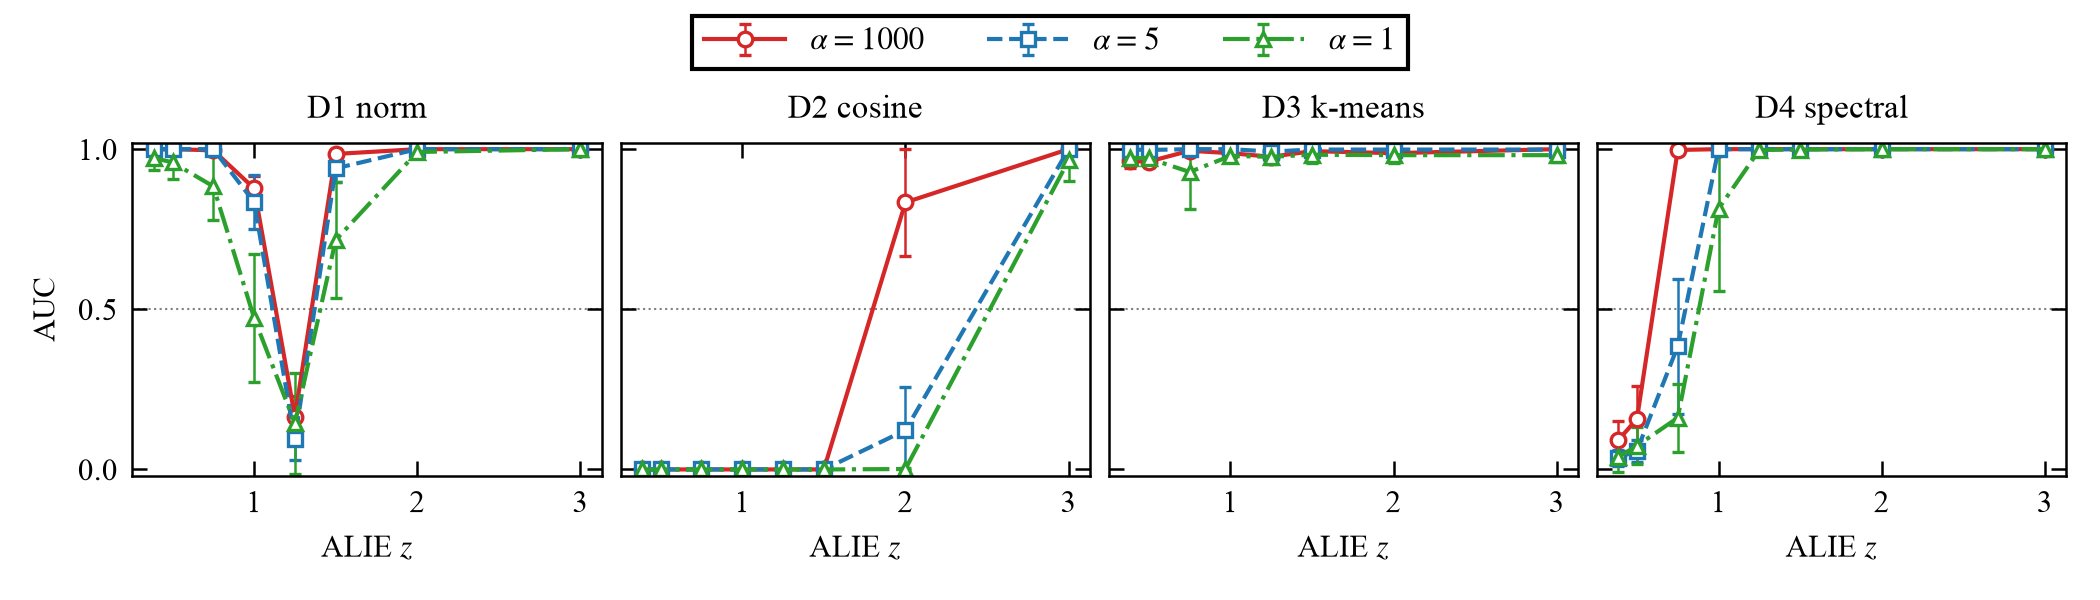
\includegraphics[width=\textwidth]{fig/detection_auc_by_z_v3.png}
\caption{ALIEの $z$ と第46--50ラウンドのAUC. 点は10試行の平均, 棒は$\pm$標準偏差. 赤実線○: $\alpha=1000$, 青破線□: $\alpha=5$, 緑一点鎖線△: $\alpha=1$. 点線は $\mathrm{AUC}=0.5$}
\label{fig:auc-z}
\end{figure*}

符号反転攻撃に対しては, D2・D3は全 $\alpha$ で $\mathrm{AUC} \ge 0.97$ であった. D1とD4は $\alpha$ が小さいほど低下し, $\alpha=1000,\,5,\,1$ の順にD1が $0.97$, $0.94$, $0.88$, D4が $1.00$, $0.97$, $0.85$ であった.

ALIEに対しては, D2は $z \le 1.5$ では全 $\alpha$ でAUCが $0.00$ であり, 順位が完全に逆転した. $z=2$ では $\alpha=1000,\,5,\,1$ の順に $0.83$, $0.12$, $0.00$, $z=3$ では全 $\alpha$ で $0.96$ 以上となった. D1のAUCは $z \le 0.5$ では全 $\alpha$ で $0.95$ 以上であり, $z=1.25$ において最小（$0.09$--$0.16$）となったのち, $z \ge 2$ では全 $\alpha$ で $0.99$ 以上であった. D3は全条件で $\mathrm{AUC} \ge 0.92$ であった. D4は $z$ が小さいと $0.04$--$0.16$ と逆転し, ある $z$ を境に $1.0$ 近くへ切り替わった. $\alpha=1000,\,5$ では切り替わりは急であり, 切り替わる $z$ はそれぞれ $0.5$ と $0.75$ の間, $0.75$ と $1$ の間にあった. $\alpha=1$ では切り替わりがなだらかであり, AUCは $z=0.75$ で $0.16$, $z=1$ で $0.81$, $z \ge 1.25$ で $1.00$ であった.

\subsection{AUCのラウンド推移}
\label{sec:res-rounds}

図\ref{fig:auc-round}に, 検知器ごとのAUCのラウンド推移（試行間の平均$\pm$標準偏差）を示す. ALIEは8水準のうち4水準のみを示す.

\begin{figure*}[t]
\centering
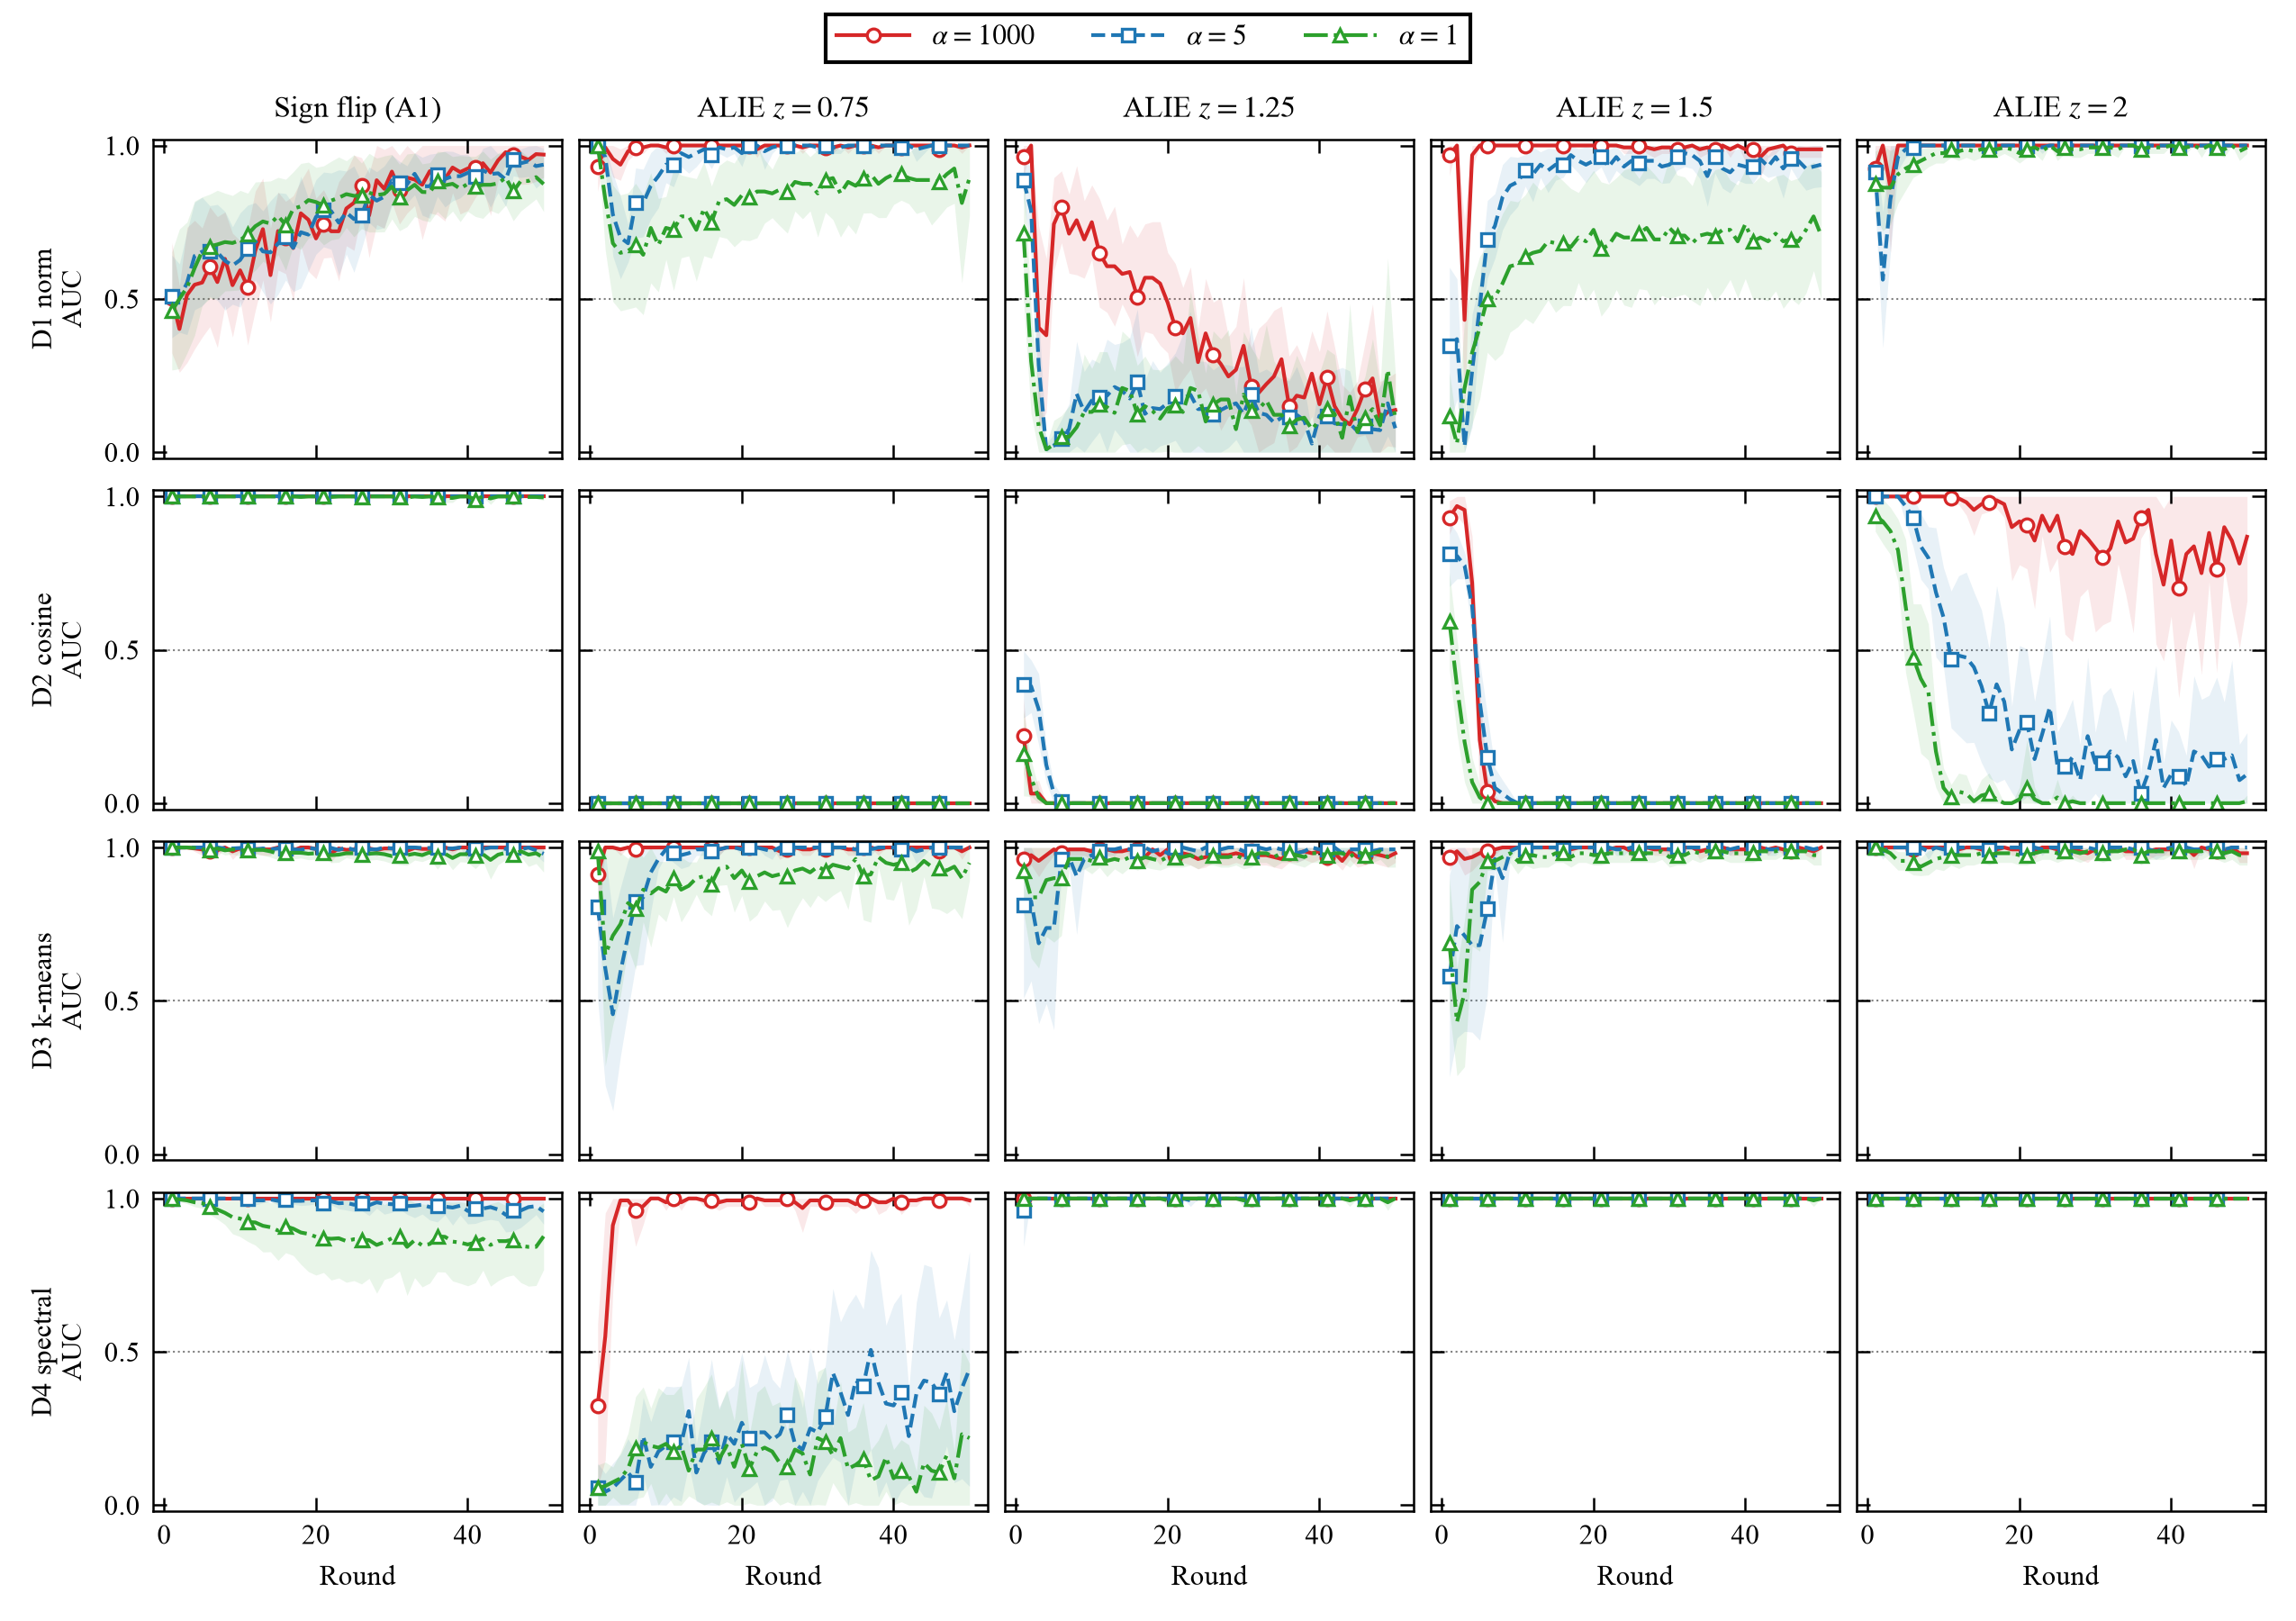
\includegraphics[width=\textwidth]{fig/detection_auc_by_round_v3_sel.png}
\caption{AUCのラウンド推移. 行は検知器D1--D4, 列は攻撃であり, ALIEは8水準のうち $z=0.75$, $1.25$, $1.5$, $2$ の4水準を示す（他の水準の第46--50ラウンドの値は表\ref{tab:final-auc}と図\ref{fig:auc-z}）. 線は試行間の平均, 帯は$\pm$標準偏差. 赤実線○: $\alpha=1000$, 青破線□: $\alpha=5$, 緑一点鎖線△: $\alpha=1$. 点線は $\mathrm{AUC}=0.5$}
\label{fig:auc-round}
\end{figure*}

符号反転では, D2は全ラウンドで $1.00$, D3は $0.97$ 以上を維持した. 一方, D1は全 $\alpha$ で学習の進行とともに上昇し（第1--5ラウンドの $0.50$--$0.57$ から第31--50ラウンドの $0.87$--$0.93$）, D4は $\alpha=1$ でのみ第1--5ラウンドの $0.99$ から第31--50ラウンドの $0.86$ へ低下した. このように, 検知性能は学習の段階によって大きく異なる場合があり, 第46--50ラウンドの値だけからは読み取れない.

\subsection{Non-IID度と正常更新のばらつき}
\label{sec:res-spread}

表\ref{tab:spread}に, 攻撃なし条件における \Spread{} と正常更新の第1主成分の寄与率を示す.

\begin{table}[t]
\centering
\begin{minipage}[t]{0.52\textwidth}
\centering
\caption{攻撃なし条件における \Spread{} と正常更新の第1主成分の寄与率. 全ラウンドの値はラウンド単位の値の平均$\pm$標準偏差}
\label{tab:spread}
\small
\begin{tabular}{@{}lcccc@{}}
\toprule
 & \multicolumn{3}{c}{\Spread{}} & 寄与率 \\
\cmidrule(lr){2-4}\cmidrule(l){5-5}
$\alpha$ & 全ラウンド & 第1--5 & 第46--50 & 第46--50 \\
\midrule
1000 & $0.151 \pm 0.009$ & $0.149$ & $0.143$ & $0.086$ \\
5    & $0.182 \pm 0.070$ & $0.353$ & $0.143$ & $0.122$ \\
1    & $0.211 \pm 0.087$ & $0.434$ & $0.155$ & $0.193$ \\
\bottomrule
\end{tabular}
\end{minipage}\hfill
\begin{minipage}[t]{0.45\textwidth}
\centering
\caption{符号反転攻撃における \PushRatio{} とAUCのSpearman順位相関係数 $\rho$（ラウンド単位, 同順位は平均順位で処理. n/a はAUCが一定で定義できないもの）}
\label{tab:corr}
\small
\begin{tabular}{@{}lcccc@{}}
\toprule
 & 全体 & $\alpha=1000$ & $\alpha=5$ & $\alpha=1$ \\
\midrule
D1 & $-0.17$ & $-0.57$ & $-0.17$ & $\phantom{-}0.69$ \\
D2 & $-0.02$ & n/a & n/a & $\phantom{-}0.06$ \\
D3 & $-0.11$ & $-0.03$ & $\phantom{-}0.07$ & $\phantom{-}0.15$ \\
D4 & $-0.32$ & n/a & $-0.19$ & $-0.12$ \\
\bottomrule
\end{tabular}
\end{minipage}
\end{table}

第1--5ラウンドでは $\alpha=1000$ の $0.149$ に対して $\alpha=5,\,1$ の \Spread{} は $0.353$, $0.434$ と約 $2.4$--$2.9$ 倍であったが, 第46--50ラウンドでは $1.00$--$1.08$ 倍にとどまった. 一方, 第1主成分の寄与率は第46--50ラウンドでも $\alpha=1000,\,5,\,1$ の順に $0.086$, $0.122$, $0.193$ と約 $2.2$ 倍の差があった.

攻撃あり条件における第46--50ラウンド平均の \PushRatio{} は, ALIEでは $\alpha$ によらず $z$ の $1.00$--$1.02$ 倍であり, 符号反転では全 $\alpha$ で $1.5$ 以上であった.

ALIEでは, 悪性方向と全更新の第1主成分の $|\cos\theta|$ がD4のAUCとよく対応した（24条件で $\rho=0.92$）. 例えば $z=0.75$ では, $|\cos\theta|$ が $\alpha=1000,\,5,\,1$ の順に $0.920$, $0.305$, $0.138$ であり, D4のAUC（$0.998$, $0.385$, $0.161$）と対応した. このときの攻撃あり条件における正常更新の第1主成分の寄与率は $0.102$, $0.141$, $0.207$ であった.

\subsection{符号反転攻撃における \PushRatio{} とAUCの関係}
\label{sec:res-pushratio}

符号反転攻撃について, \PushRatio{} とAUCのSpearman順位相関係数 $\rho$ を表\ref{tab:corr}に示す. 相関は, 1回の実行の1ラウンドを1点とし, 検知器ごとに全体（$1{,}500$ 点）と $\alpha$ ごと（各 $500$ 点）で求めた.



両者の順位相関は, 全体でも $\alpha$ ごとでも弱いか負であり, 例外は $\alpha=1$ のD1（$\rho=0.69$）のみであった.

\section{考察}
\label{sec:discussion}

\subsection{検知器間の違い}
\label{sec:disc-detectors}

符号反転攻撃に対しては, D2とD3が全 $\alpha$ で高い検知性能を示した（表\ref{tab:final-auc}）. これは, 正常更新が共通の方向を持つためと考えられる. 正常更新 $g$ と参照方向 $r$ のなす角を $\theta$ とすると, D2スコアは正常更新で $1-\cos\theta$, 符号を反転した悪性更新で $1+\cos\theta$ となる. したがって, $\cos\theta>0$ である限り, 両者の順位は必ず分かれる. 実際, 第1--5ラウンドのスコアの平均は, $\alpha=1000$ で正常更新が $0.04$, 悪性更新が $1.95$ であった（図\ref{fig:signflip-d2}）. D3もD2スコアを特徴量に含み, 悪性方向と全更新の第1主成分の $|\cos|$ は全 $\alpha$ で $0.96$ 以上であったため, 同じ性質によって分離されやすい. ただし, 学習が進むと正常更新の向きが揃わなくなり, 両者のスコアは $1$ に近づいた（$\alpha=1000$ の第46--50ラウンドで正常更新が $0.74$, 悪性更新が $1.16$）.

\begin{figure}[t]
\centering
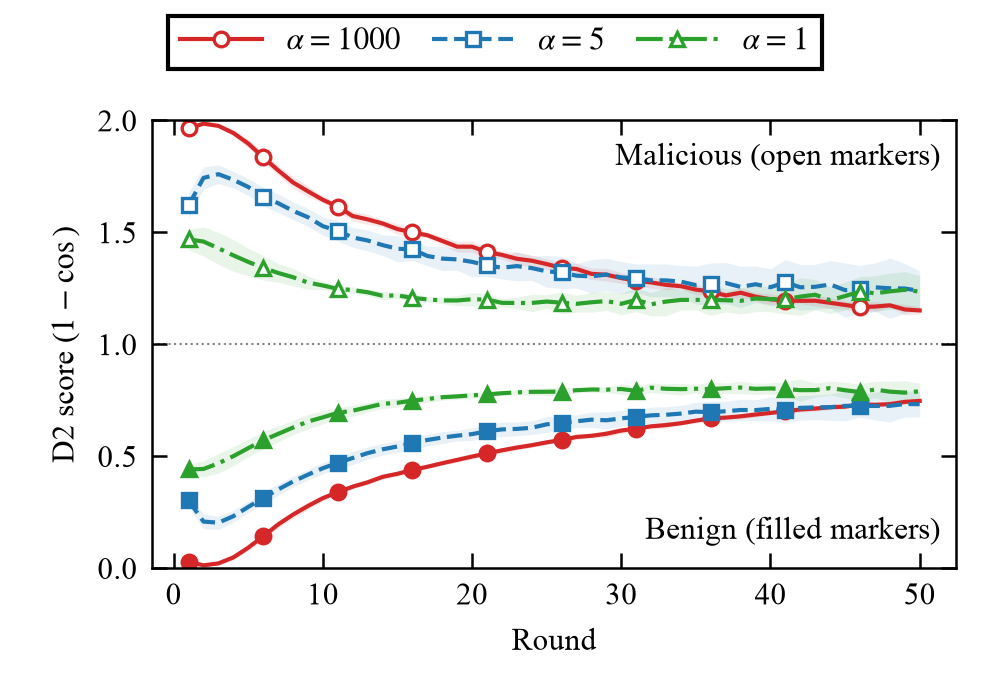
\includegraphics[width=0.5\textwidth]{fig/signflip_d2_score_by_round_v3.png}
\caption{符号反転攻撃におけるD2スコア（参照方向へのコサイン距離）のラウンド推移. 白抜きの印は悪性更新, 塗りつぶしの印は正常更新の平均を表す（10試行の平均, 帯は$\pm$標準偏差）. 赤実線○: $\alpha=1000$, 青破線□: $\alpha=5$, 緑一点鎖線△: $\alpha=1$. 点線は $\cos\theta=0$ に対応するスコア $1$}
\label{fig:signflip-d2}
\end{figure}

ALIEに対しては, D2のAUCは $z \le 1.5$ のすべての条件で $0.00$ であった（表\ref{tab:final-auc}）. これは, すべての悪性更新がすべての正常更新よりも正常らしいと判定され, 順位が完全に逆転していることを意味する. D2の参照方向 $r$ は全更新の座標ごとの中央値であり, 4台の悪性更新はすべて同じベクトルで, どの座標でも平均より下の同じ側に位置するため, $r$ は悪性更新の側へ寄る. 一方, 正常更新の各クライアントのずれは座標ごとに向きがばらばらであり, 高次元では悪性方向とほぼ直交する. そのため, 正常更新のD2スコアはほぼ $1$ となり, 悪性更新のスコア（$z=1$ で $0.22$--$0.33$）を上回った.

D3は, ALIEに対してもすべての条件でAUC $0.92$ 以上を示した. D3のスコアは正常クラスタの重心からの距離であり, どちらの向きに外れても大きくなるため, D2で順位の逆転を招いた外れ方も検出される. 加えて, ALIEでは悪性クライアント4台が同一のベクトルを送るため, 悪性更新は特徴量の空間で1点に重なり, 分離されやすい.

以上より, 第一の問いに対しては次のようにいえる. 検知器の優劣は攻撃によって入れ替わり, 検知の成否は, 攻撃が悪性更新をどこに置くかと, 検知器がどの量を見て, どの向きの外れを異常とみなすかの組み合わせによって決まる.

\subsection{Non-IID度が検知性能に与える影響}
\label{sec:disc-noniid}

Non-IIDは検知性能を低下させたが, その低下は, 中心仮説が予測した正常更新のばらつきの大きさ \Spread{} の増大では説明できない. \Spread{} は学習の序盤には $\alpha$ が小さいほど大きかった（第1--5ラウンドで $\alpha=1000$ の約 $2.4$--$2.9$ 倍）が, 第46--50ラウンドでは $1.00$--$1.08$ 倍とほとんど差がなかった（表\ref{tab:spread}）. 一方, 検知性能が $\alpha$ によって大きく異なったのは主に学習の後半であった.

代わりに検知性能の低下と対応していたのは, ばらつきの配分であった. 第一に, Non-IIDは正常更新のノルムのばらつきを大きくし（符号反転の第46--50ラウンドにおける変動係数は $\alpha=1000,\,5,\,1$ の順に $0.08$, $0.17$, $0.39$）, ノルムに依存するD1とD4の符号反転に対する検知性能を低下させた. 第二に, Non-IIDは各クライアントの更新を異なる向きに向けるため, 共通の成分が各クライアントのずれに比べて小さくなり, ALIEに対してD2が検知に転じる $z$ を大きくした（$\alpha=1000$ では $z=2$, $\alpha=1$ では $z=3$）. 第三に, Non-IIDは正常更新のばらつきを特定の方向に集中させた. ALIEの $z=0.75$ では \PushRatio{} がいずれの $\alpha$ でも約 $0.75$ であるにもかかわらず, D4のAUCは $\alpha=1000,\,5,\,1$ の順に $1.00$, $0.39$, $0.16$ であり, 正常更新の第1主成分の寄与率（$0.102$, $0.141$, $0.207$. \ref{sec:res-spread}節）が大きいほど低かった.

以上より, 第二の問いに対しては次のようにいえる. Non-IIDは検知性能を低下させるが, その低下は \Spread{} の増大では説明できず, ばらつきの配分と対応していた. Liら（2023）\cite{li2023experimental}は, Non-IIDが複数のRobust Aggregation手法の頑健性を最終精度の観点で低下させることを報告している. 本結果はこれと矛盾せず, 同じ現象を検知性能の観点から評価し, その低下が正常更新の分布の形と対応することを示した点で, Liら（2023）の結果を補うものである.

\subsection{攻撃のステルス性と検知破綻の境界}
\label{sec:disc-rq3}

中心仮説は, \PushRatio{} が $1$ を下回ると検知性能が急落すると予測した. ALIEでは $\PushRatio \approx z$ であるため, $z<1$ の水準がこの領域に対応する. しかし, 最も内側の $z=0.385$ でも, D1とD3は全 $\alpha$ でAUC $0.96$ 以上で悪性更新を検知した（表\ref{tab:final-auc}）.

この結果は, 高次元空間における正常更新の配置から説明できる. 正常更新の平均からの距離の2乗は約26万個の正の値の和であるため, 正常更新どうしでほぼ同じ値に集中すると考えられる. 実際, 正常更新の平均からの距離の変動係数は, 第46--50ラウンドで $\alpha=1000,\,5,\,1$ の順に約 $0.08$, $0.09$, $0.18$ であった. すなわち, 正常更新は平均からほぼ一定の距離の薄い殻の上に並んでおり, 平均の近くにはほとんど存在しない. そのため, $z=0.385$ の悪性更新は殻の内側に位置し, 平均に近すぎることによって正常更新から区別される. ただし, この解釈は結果を見たあとに整理したものである.

\begin{figure*}[t]
\centering
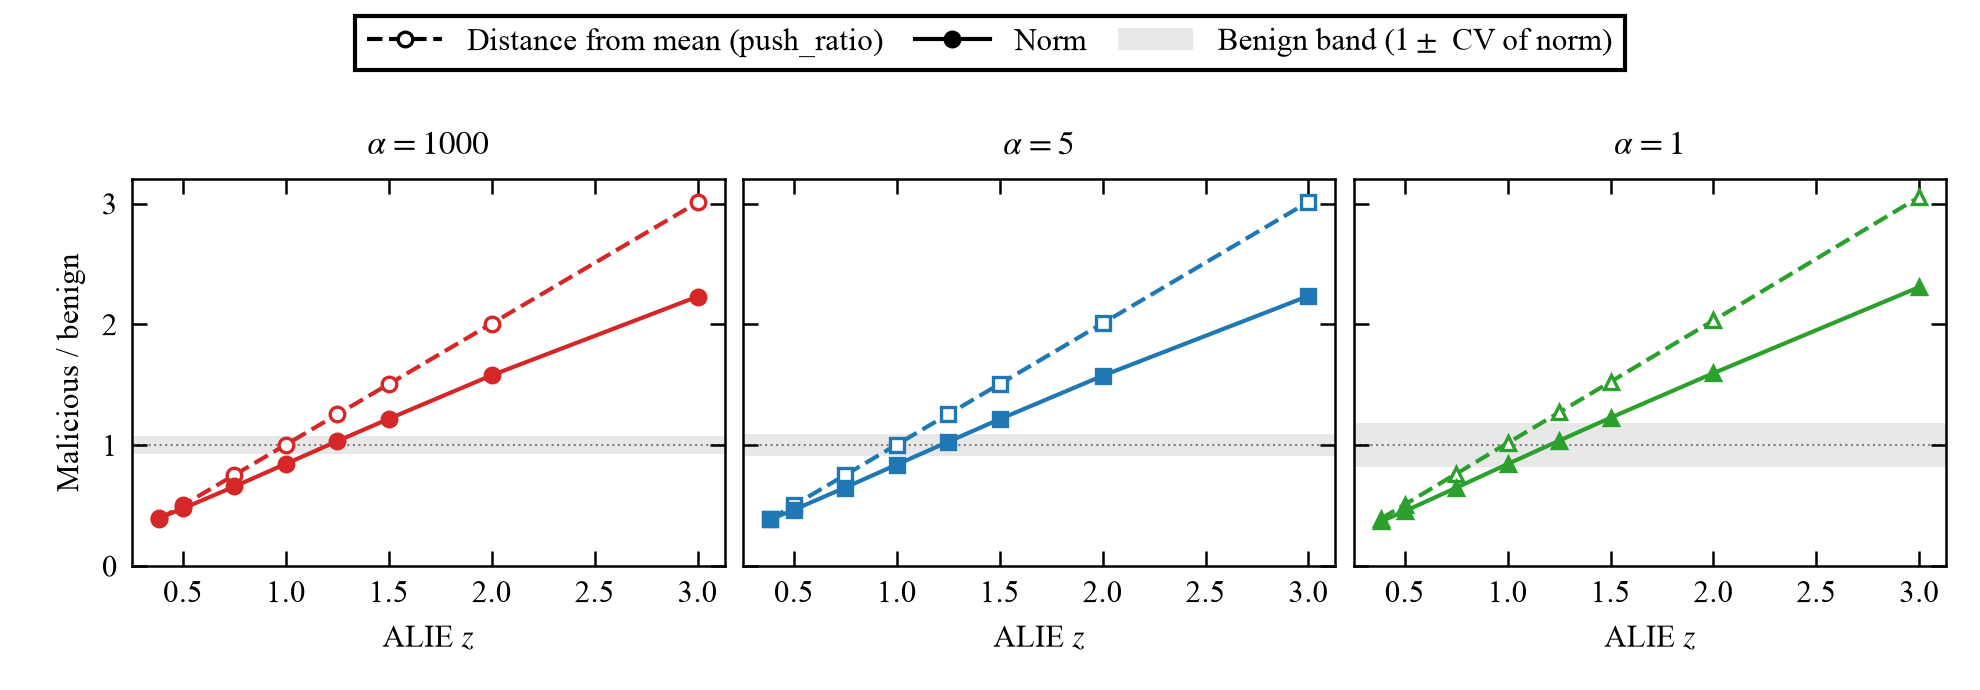
\includegraphics[width=0.85\textwidth]{fig/alie_shell_by_z_v3.png}
\caption{ALIEの $z$ と, 悪性更新の正常更新に対する比（第46--50ラウンド, 10試行の平均）. 破線（白抜きの印）は平均からの距離の比（\PushRatio{}）, 実線（塗りつぶしの印）はノルムの比. 灰色の帯は $1 \pm$ 正常更新のノルムの変動係数であり, 正常更新の殻の厚みの目安を表す. 点線は比 $1$}
\label{fig:alie-shell}
\end{figure*}

$z$ を大きくすると, 悪性更新は殻に近づき, さらに大きくすると殻の外に出る（図\ref{fig:alie-shell}）. そのため, 距離やノルムに基づく検知が最も困難になるのは, 悪性更新が殻の上に来る付近である. 実際, D1のAUCは全 $\alpha$ で, 悪性更新のノルムが正常更新と揃う $z=1.25$ において最小（$0.09$--$0.16$）となり, $z \ge 2$ で再び $0.99$ 以上となった.

以上より, 第三の問いに対しては次のようにいえる. 悪性更新を正常更新の平均に近づけることは, 検知を回避する手段にはならない. $\PushRatio=1$ は検知が破綻する境界ではなく, 悪性更新が殻の上に来て, 距離やノルムに基づく検知から最も隠れやすくなる点の近くである.

\subsection{中心仮説の評価}
\label{sec:disc-hyp}

中心仮説は, (1) Non-IIDは \Spread{} を増大させる, (2) 検知可能性は \PushRatio{} でほぼ決まり, $1$ を下回ると検知性能が急落する, (3) したがってNon-IIDは検知性能を低下させる, という3つの主張からなる. (1)は学習の序盤には成り立ったが, 学習が進んだ段階ではほとんど成り立たなかった（\ref{sec:disc-noniid}節）. (2)は支持されなかった. 符号反転では \PushRatio{} とAUCの順位相関は全体で $-0.32$--$-0.02$ であり, 正の相関は見られなかった（表\ref{tab:corr}）. また, ALIEでは $z<1$ でも検知性能は急落せず（\ref{sec:disc-rq3}節）, $z=0.75$ では同じ \PushRatio{} でもD4のAUCが $\alpha$ によって大きく異なった（\ref{sec:disc-noniid}節）. (3)は観測されたが, その理由は \Spread{} の増大ではなく, ばらつきの配分であった.

仮説が外れた原因は, 主に2つあると考えられる. 第一に, 中心仮説は, 正常更新が平均の周りを埋めるという低次元の直感に基づいていた. 実際には, 高次元の正常更新は平均からほぼ一定の距離の殻の上に並ぶため, 平均に近い悪性更新はむしろ目立った. 第二に, \PushRatio{} は悪性更新の位置を「正常更新の平均からの距離」という1つの量にまとめたものであるが, 検知器はそれぞれ異なる量を見て, 異なる向きの外れを異常とみなす. そのため, 検知可能性を説明するには, 検知器が見る量の上での悪性更新の位置と, 正常更新の分布の形を考慮する必要がある.

なお, 本研究のALIEの多くはFedAvgのもとで精度をほとんど低下させておらず, 本研究の結果は主に検知性能に関するものである. また, 実験はMNIST, 20台のクライアント, ラベルの偏りのみのNon-IIDという限られた条件で行った.

\section{おわりに}
\label{sec:conclusion}

本研究では, FLにおける悪性更新の検知可能性を, データ分布の不均一性（Non-IID度）と攻撃のステルス性の2つの観点から, 4種類の検知器のROC-AUCにより評価した. その結果, 検知できるかどうかは, 悪性更新が検知器の見る量の上でどこに位置し, 検知器がどの向きの外れを異常とみなすかによって決まっていた. また, Non-IIDは検知性能を低下させたが, その原因は正常更新のばらつきの大きさではなく, ばらつきの配分であった. したがって, 悪性更新の押し出し量と正常更新のばらつきの比で検知可能性がほぼ決まるという中心仮説は支持されなかった.

{\small
\begin{thebibliography}{99}

\bibitem{mammen2021fl}
Priyanka Mary Mammen,
``Federated Learning: Opportunities and Challenges,''
arXiv preprint arXiv:2101.05428, 2021.

\bibitem{sagar2023survey}
Subhash Sagar, Chang-Tsun Li, Seng W. Loke, Jinho Choi,
``Poisoning Attacks and Defenses in Federated Learning: A Survey,''
arXiv preprint arXiv:2301.05795, 2023.

\bibitem{baruch2019little}
Gilad Baruch, Moran Baruch, Yoav Goldberg,
``A Little Is Enough: Circumventing Defenses For Distributed Learning,''
Advances in Neural Information Processing Systems (NeurIPS), 2019.

\bibitem{li2023experimental}
Shenghui Li, Edith C.-H. Ngai, Thiemo Voigt,
``An Experimental Study of Byzantine-Robust Aggregation Schemes in Federated Learning,''
arXiv preprint arXiv:2302.07173, 2023.

\bibitem{fang2020local}
Minghong Fang, Xiaoyu Cao, Jinyuan Jia, Neil Zhenqiang Gong,
``Local Model Poisoning Attacks to Byzantine-Robust Federated Learning,''
Proceedings of the 29th USENIX Security Symposium (USENIX Security 2020),
pp.~1605--1622, 2020.

\bibitem{blanchard2017krum}
Peva Blanchard, El Mahdi El Mhamdi, Rachid Guerraoui, Julien Stainer,
``Machine Learning with Adversaries: Byzantine Tolerant Gradient Descent,''
Advances in Neural Information Processing Systems (NeurIPS), 2017.

\bibitem{yin2018byzantine}
Dong Yin, Yudong Chen, Kannan Ramchandran, Peter Bartlett,
``Byzantine-Robust Distributed Learning: Towards Optimal Statistical Rates,''
Proceedings of the 35th International Conference on Machine Learning (ICML), 2018.

\bibitem{elmhamdi2018hidden}
El Mahdi El Mhamdi, Rachid Guerraoui, S\'ebastien Rouault,
``The Hidden Vulnerability of Distributed Learning in Byzantium,''
Proceedings of the 35th International Conference on Machine Learning (ICML), 2018.

\bibitem{shejwalkar2021manipulating}
Virat Shejwalkar, Amir Houmansadr,
``Manipulating the Byzantine: Optimizing Model Poisoning Attacks and Defenses for Federated Learning,''
Network and Distributed System Security Symposium (NDSS), 2021.

\bibitem{nguyen2022flame}
Thien Duc Nguyen et al.,
``FLAME: Taming Backdoors in Federated Learning,''
31st USENIX Security Symposium (USENIX Security 2022), pp.~1415--1432, 2022.

\bibitem{hsu2019measuring}
Tzu-Ming Harry Hsu, Hang Qi, Matthew Brown,
``Measuring the Effects of Non-Identical Data Distribution for Federated Visual Classification,''
arXiv preprint arXiv:1909.06335, 2019.

\bibitem{li2022federated}
Qinbin Li, Yiqun Diao, Quan Chen, Bingsheng He,
``Federated Learning on Non-IID Data Silos: An Experimental Study,''
Proceedings of the 38th IEEE International Conference on Data Engineering (ICDE), 2022.

\bibitem{wang2023trust}
Zhilin Wang, Qin Hu, Xukai Zou,
``Can We Trust the Similarity Measurement in Federated Learning?,''
arXiv preprint arXiv:2311.03369, 2023.

\bibitem{cao2021fltrust}
Xiaoyu Cao, Minghong Fang, Jia Liu, Neil Zhenqiang Gong,
``FLTrust: Byzantine-robust Federated Learning via Trust Bootstrapping,''
Network and Distributed System Security Symposium (NDSS), 2021.

\bibitem{shejwalkar2022back}
Virat Shejwalkar, Amir Houmansadr, Peter Kairouz, Daniel Ramage,
``Back to the Drawing Board: A Critical Evaluation of Poisoning Attacks on Production Federated Learning,''
IEEE Symposium on Security and Privacy (S\&P), 2022.

\bibitem{mcmahan2017fedavg}
H.~Brendan McMahan, Eider Moore, Daniel Ramage, Seth Hampson, Blaise Aguera y Arcas,
``Communication-Efficient Learning of Deep Networks from Decentralized Data,''
Proceedings of the 20th International Conference on Artificial Intelligence and Statistics (AISTATS),
pp.~1273--1282, 2017.

\bibitem{shen2016auror}
Shiqi Shen, Shruti Tople, Prateek Saxena,
``Auror: Defending Against Poisoning Attacks in Collaborative Deep Learning Systems,''
Proceedings of the 32nd Annual Conference on Computer Security Applications (ACSAC), 2016.

\bibitem{tran2018spectral}
Brandon Tran, Jerry Li, Aleksander Madry,
``Spectral Signatures in Backdoor Attacks,''
Advances in Neural Information Processing Systems (NeurIPS), 2018.

\bibitem{fawcett2006roc}
Tom Fawcett,
``An Introduction to ROC Analysis,''
Pattern Recognition Letters, vol.~27, no.~8, pp.~861--874, 2006.

\bibitem{hanley1982meaning}
James A. Hanley, Barbara J. McNeil,
``The Meaning and Use of the Area under a Receiver Operating Characteristic (ROC) Curve,''
Radiology, vol.~143, no.~1, pp.~29--36, 1982.

\bibitem{beutel2020flower}
Daniel J. Beutel, Taner Topal, Akhil Mathur, Xinchi Qiu, Javier Fernandez-Marques, Yan Gao, Lorenzo Sani, Kwing Hei Li, Titouan Parcollet, Pedro Porto Buarque de Gusm\~{a}o, Nicholas D. Lane,
``Flower: A Friendly Federated Learning Research Framework,''
arXiv preprint arXiv:2007.14390, 2020.

\end{thebibliography}
}

\end{document}
